\documentclass{article}

% if you need to pass options to natbib, use, e.g.:
% \PassOptionsToPackage{numbers, compress}{natbib}
% before loading nips_2016
%
% to avoid loading the natbib package, add option nonatbib:
%\usepackage[nonatbib]{nips_2016}

%\usepackage{nips}

% to compile a camera-ready version, add the [final] option, e.g.:
\usepackage[final]{nips_2016}

\usepackage[utf8]{inputenc} % allow utf-8 input
\usepackage[T1]{fontenc}    % use 8-bit T1 fonts
\usepackage{hyperref}       % hyperlinks
\usepackage{url}            % simple URL typesetting
\usepackage{booktabs}       % professional-quality tables
\usepackage{amsfonts}       % blackboard math symbols
\usepackage{nicefrac}       % compact symbols for 1/2, etc.
\usepackage{microtype}      % microtypography

\usepackage{amssymb}
\usepackage{mathtools}
\usepackage{latexsym}
\usepackage{amsthm}
\usepackage{enumerate}
\usepackage{epsfig}
\usepackage{graphicx}
\usepackage{color}
\usepackage{float}
\usepackage{subfigure}
\usepackage{amsmath}
\usepackage{MnSymbol}
\usepackage{makeidx}
\usepackage{fancyhdr}
\usepackage{relsize}
\pagestyle{fancy}
\usepackage{lastpage}
\usepackage{url}
\usepackage{mathrsfs}

\newcommand{\F}{\ensuremath{\mathcal F}}
\DeclareMathSymbol{\R}{\mathbin}{AMSb}{"52}
\newcommand{\f}{\ensuremath{\mathcal f}}
\newcommand{\C}{\ensuremath{\mathcal C}}
\newcommand{\M}{\ensuremath{\mathcal M}}
\renewcommand{\H}{\ensuremath{\mathcal H}}
\newcommand{\pisys}{\ensuremath{\mathscr{L}}}
\newcommand{\lsys}[1]{\ensuremath{\lambda \lp #1 \rp}}
\newcommand{\A}{\ensuremath{\mathcal A}}
\newcommand{\E}{\ensuremath{\mathcal E}}
\renewcommand{\L}{\ensuremath{\mathcal L}}
\newcommand{\norm}[1]{\ensuremath{\mathcal \| #1 \|}}
\newcommand{\Exp}[1]{\ensuremath{\mathbb{E} \lb #1 \rb}}
\newcommand{\condExp}[2]{\ensuremath{\mathbb{E} \lb #1 | #2 \rb}}
\newcommand{\lp}{\ensuremath{\left(}}
\newcommand{\rp}{\ensuremath{\right)}}
\newcommand{\lb}{\ensuremath{\left[}}
\newcommand{\rb}{\ensuremath{\right]}}
\newcommand{\B}[1]{\ensuremath{\mathcal B\lp #1 \rp}}
\newcommand{\Pset}[1]{\ensuremath{\mathcal P\lp #1 \rp}}
\newcommand{\siga}[1]{\ensuremath{\sigma\lp #1 \rp}}
\newcommand{\Xrv}[1]{\ensuremath{X\lp #1 \rp}}
\newcommand{\Xrvi}[1]{\ensuremath{X \inv \lp #1 \rp}}
\newcommand{\Yrv}[1]{\ensuremath{Y\lp #1 \rp}}
\newcommand{\Prob}[1]{\ensuremath{\Pb\lp #1 \rp}}
\newcommand{\inv}{\ensuremath{^{-1}}}
\newcommand{\iprod}[2]{\ensuremath{\llangle #1, #2 \rrangle}}
\newcommand{\twopartdef}[4]
{
	\left\{
		\begin{array}{ll}
			#1 & \mbox{if } #2 \\
			#3 & \mbox{if } #4
		\end{array}
	\right.
}
\newcommand\independent{\protect\mathpalette{\protect\independenT}{\perp}}
\def\independenT#1#2{\mathrel{\rlap{$#1#2$}\mkern2mu{#1#2}}}

\title{Prior Formulation for Gaussian Process Hyperparameters}

% The \author macro works with any number of authors. There are two
% commands used to separate the names and addresses of multiple
% authors: \And and \AND.
%
% Using \And between authors leaves it to LaTeX to determine where to
% break the lines. Using \AND forces a line break at that point. So,
% if LaTeX puts 3 of 4 authors names on the first line, and the last
% on the second line, try using \AND instead of \And before the third
% author name.

\author{
  Rob Trangucci \\
  Applied Statistics Center\\
  Columbia University\\
  New York, NY 10027 \\
  \texttt{robert.trangucci@gmail.com} \\
%	\and
%	  Michael Betancourt \\
%	  Applied Statistics Center\\
%	  Columbia University\\
%	  New York, NY 10027 \\
%	  \texttt{betanalpha@gmail.com} \\
}

\author{
  Rob Trangucci \\
  Applied Statistics Center\\
  Columbia University\\
  New York, NY 10027 \\
  \texttt{rnt2101@columbia.edu} \\
}

\begin{document}
% \nipsfinalcopy is no longer used

\maketitle

\begin{abstract}
  Gaussian processes are measures over functions, and as such, can be used as a
  rich prior for latent functions in Bayesian statistical models. However, the
  joint posterior density of the length scale and marginal variance
  hyperparameters in stationary kernels like the exponentiated quadratic and
	M\'{a}tern is often weakly informed by the data because of the extreme
  flexibility of Gaussian process priors. We develop a principled approach for
  specifying weakly informative priors for length scale hyperparameters that impose
  soft constraints on the space of functions represented by the Gaussian
  process prior.
\end{abstract}


\section{Introduction}

As noted by many authors (\citet{flaxman2015fast},
\citet{stein2012interpolation}, \citet{rasmussen2006gaussian},
\citet{fuglstad2015interpretable}), learning hyperparameters in Gaussian process
(GP) kernels is notoriously hard. The preponderance of literature has focused
estimating hyperparameters using marginal maximum likelihood for point
estimation (\citet{stein2012interpolation}, \citet{rasmussen2006gaussian}), and
the asymptotic properties of posterior conditional mean functions in GP
regressions (\citet{seeger2008information}, \citet{stein2012interpolation},
\citet{rasmussen2006gaussian}, \citet{williams2000upper}). As applied
statisticians, we want to allow for flexibility in our priors over latent
functions, given that we will select the wrong posterior latent function using
one set of parameters with probability one for finite data. Thus, instead of
picking one set of hyperparameters, we would like to place priors over
hyperparameters and integrate over our uncertainty when making predictions for
new data. For maximum flexibility in model building, we would like to select
uninformative priors, run our MCMC chains to convergence, and calculate
posterior expectations for our estimands of interest. 

Unfortunately, uninformative priors or weakly informative priors
can yield large posterior intervals for hyperparameters and lead to wide
posterior predictive intervals when data are not informative about model
parameters (\citet{fuglstad2015interpretable}). Thus, we need a better
understanding of how weakly informative priors interact with the likelihood
under a Gaussian process prior.

In order to gain insight into the empirical behavior of different priors, we
explore how efficiently 4 weakly informative priors can extract known
parameters in 12 different data generating processes, using techniques from
\citet{cook2012validation}. We chose to study the deliberately simple 1-D
Gaussian process regression model in order to elucidate the pathologies
inherent in posterior inference over kernel hyperparameters.

In section \ref{background} we define the 1-D Gaussian process regression setting,
the hyperparameters of interest, and the mathematical basis for the manifestations
of weak identifiability in kernel hyperparameters. In section \ref{experiment}, we 
outline the experimental set up, and in section \ref{results} we discuss the results 
of our experiments. Stan code is presented in the appendix.

\section{Background} \label{background}

The typical regression setting for observed univariate data, as presented in \citet{flaxman2015fast},

$y_i \in \R, x_i \in \R^M\, i \in {1,\dots,n}$:

\begin{align*}
  \theta & \sim g(\phi) \\
  f(x) & \sim \text{GP}\lp \mu(x),
  K_\theta(x, x) \rp \\
  y_i & \sim \mathcal{N}\lp f(x_i), \delta \rp \forall i \\
\end{align*}

where $\text{GP}$ is a stochastic process from which finite-sample realizations are
multivariate Gaussian, and which is completely specified its mean vector $\mu$
and its covariance matrix $K_\theta(x, x)$. The $i, j$ th
element of $K_\theta(x, x)$:

\[
  \text{cov}(f(x_i), f(x_j)) = k(x_i, x_j | \theta) 
\]

We focus on the squared exponential kernel, where $\theta$ comprises
two hyperparameters, $\ell$, the length-scale, and $\alpha$, the marginal
standard deviation:

\[ \label{kern}
  k(x_i, x_j) = \alpha^2 
\exp \left(
	- \dfrac{1}{2\ell^2} (x_{i} - x_{j})^2
\right)
\]

With $\ell$ and $\alpha$ fixed, inference of $f(x | \, \mathbf{y}, \theta)$ is
straightforward, with $f$ and $\mathbf{y}$ jointly normally distributed:
%put arrow above y and x to indicate vector of x and y $$:

\begin{align*} \begin{pmatrix} f\\ \mathbf{y} \\ \end{pmatrix} \sim
\mathcal{N} \lp \begin{pmatrix} \mathbf{0} \\ \mathbf{0} \end{pmatrix} ,\,\,
  \begin{pmatrix} K_\theta &
  K_\theta  \\ K_\theta &
  K_\theta + \delta ^ 2 \mathbf{I}\\ \end{pmatrix} \rp
\end{align*}

We can derive $p(f | \mathbf{y})$ from the properties of the joint normal
distribution: 

\begin{align*}
  f \sim
  \mathcal{N}(K_\theta  (K_\theta +
  \delta ^ 2 \mathbf{I})^{-1}\mathbf{y},  
  K_\theta - K_\theta (K_\theta + \delta ^ 2 \mathbf{I})^{-1}K_\theta)
\end{align*}

Out-of-sample predictions are generated similarly:

\begin{align*} 
  \mathbf{\tilde{y}} \sim
  \mathcal{N}(&K_\theta(\mathbf{\tilde{x}},\mathbf{x}), (K_\theta(\mathbf{x},\mathbf{x}) +
  \delta ^ 2 \mathbf{I})^{-1}\mathbf{y},  
   \\ & K_\theta(\mathbf{\tilde{x}},\mathbf{\tilde{x}}) -K_\theta(\mathbf{\tilde{x}},\mathbf{x}) (K_\theta(\mathbf{x},\mathbf{x}) + \delta ^ 2 \mathbf{I})^{-1}K_\theta(\mathbf{x},\mathbf{\tilde{x}}) + \delta ^ 2 \mathbf{I})
\end{align*}

However, if we want to infer $\theta$ from the data we will need to take our
uncertainty in $\theta$ into account. We can see that both $\ell$ and $\alpha$
will impact our predictions for $\tilde{\mathbf{y}}$.  $\alpha^2$ controls the
marginal variance of the stochastic process. For a fixed noise variance,
$\delta^2$, increasing the marginal variance of the stochastic process
increases the signal-to-noise ratio, $\alpha^2 / \delta^2$ (SN). $\ell$ controls the process's
nonlinearity. \ref{prior_lat_draws} shows the difference between draws from a GP prior
with a large $\ell$ and draws from a GP prior with a small $\ell$.

Naturally, $\ell$ and $\alpha$ also control observable statistics of the
process like the expected number of crossings of $f(x)$ on the interval $[0,
T]$ at level $u$, $C_u$. \citet{cramer2004stationary} show that $\Exp{C_u}$:

\[ 
  \Exp{C_u | \theta} = \dfrac{T}{\pi} 
\sqrt{-\dfrac{k_\theta^{\prime \prime}(0)}{k_\theta(0)}}
  \text{exp}\left(-\dfrac{u^2}{2k_\theta(0)}\right)
\]

For the $\Exp{C_u}$ exponentiated quadratic kernel:

\[ 
  \Exp{C_u | \alpha, \ell} = \dfrac{T}{\pi \ell}\text{exp}\left(-\dfrac{u^2}{2 \alpha ^ 2} \right)
\]

We can see that at $u = 0$, we are left with $\Exp{C_u} = T / \pi \ell$.  

\begin{figure}[h] \label{prior_lat_draws}
  \centering
  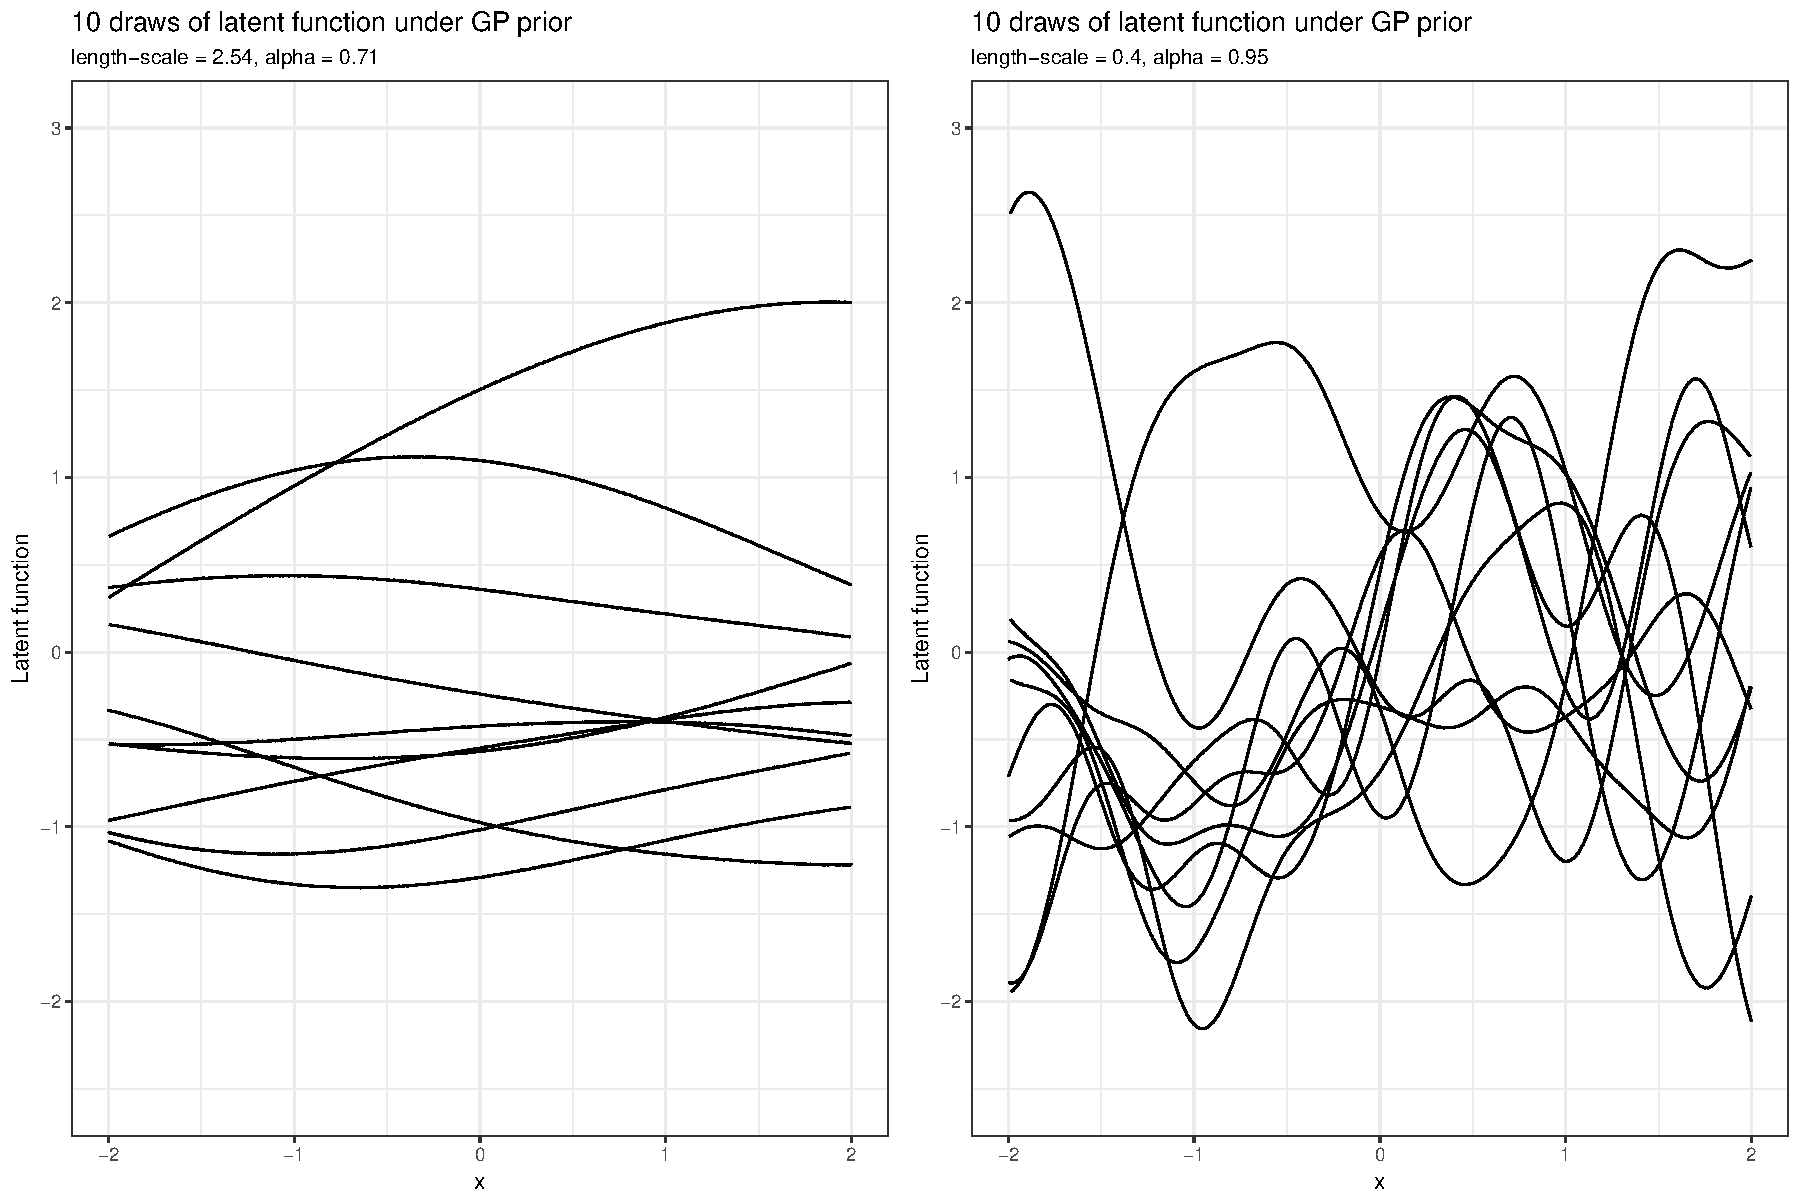
\includegraphics[width=100mm]{plots/latent_draws_comparison.pdf}
  \caption{Parameters which lead to expected zero crossings of 1/2 on left and 3.16 crossings on right}
\end{figure}

However, at $u \neq 0$ we can see that $\alpha$ and $\ell$ are conflated in
$\Exp{C_u}$. This is due to the weak identifiability of the marginal standard
deviation parameter, $\alpha$, and the length scale parameter, $\ell$, driven 
by the Gaussian process prior with an exponentiated quadratic kernel.

The weak identifiability also arises in the power spectrum of this kernel,
derived in \citet{rasmussen2006gaussian}:

\[
  S(s) \propto \alpha^2 \ell
   \exp \left(
  - 2 \pi^2 \ell^2 s^2
\right)
\]

The $\alpha ^ 2 \ell$ term drives the exponentiated quadratic kernel's
nonidentifiability. As this is a multiplicative nonidentifiability we would
expect that this would lead to positive posterior correlation between $\alpha$
and $\ell$. However, it is not clear whether using strong independent prior
information will mitigate this posterior correlation, nor is it clear how weak
priors over $\ell$ will manifest themselves in posteriors over $\alpha$. 

Turning to \ref{kern} again, we can see that the limiting behavior of the GP
as $\ell \rightarrow \infty$ and $\alpha \rightarrow 0$ each lead to the constant
function. We can also see that $\ell \rightarrow 0$ will conflate inferences in $\delta$.
Note that as $\ell \rightarrow 0$ $\Exp{C_u}$ diverges.   

\section{Experiment} \label{experiment}

We investigate the properties of posterior inferences under several prior
formulations by generating 100 datasets for 12 data generating processes and
subsequently inferring $\alpha$, $\ell$, and $\delta$ by using Stan.

\subsection{Priors}

Our intuition is that limiting behavior of GPs was an important driver of weak
identifiability, so we calibrated our choices of priors for $\ell$ by fixing
the amount of probability mass between 0 and 1 for each prior at $\sim60\%$ but
by varying the priors' mass near zero and by varying the priors' tail
heaviness.

This yields 4 priors: $\text{Gamma}(2, 2)$, $\text{Half-Cauchy}(0, 0.7)$,
$\text{Half-Normal}(0, 1.2)$, $\text{Weibull}(2, 1)$

\begin{figure}[h]
  \centering
  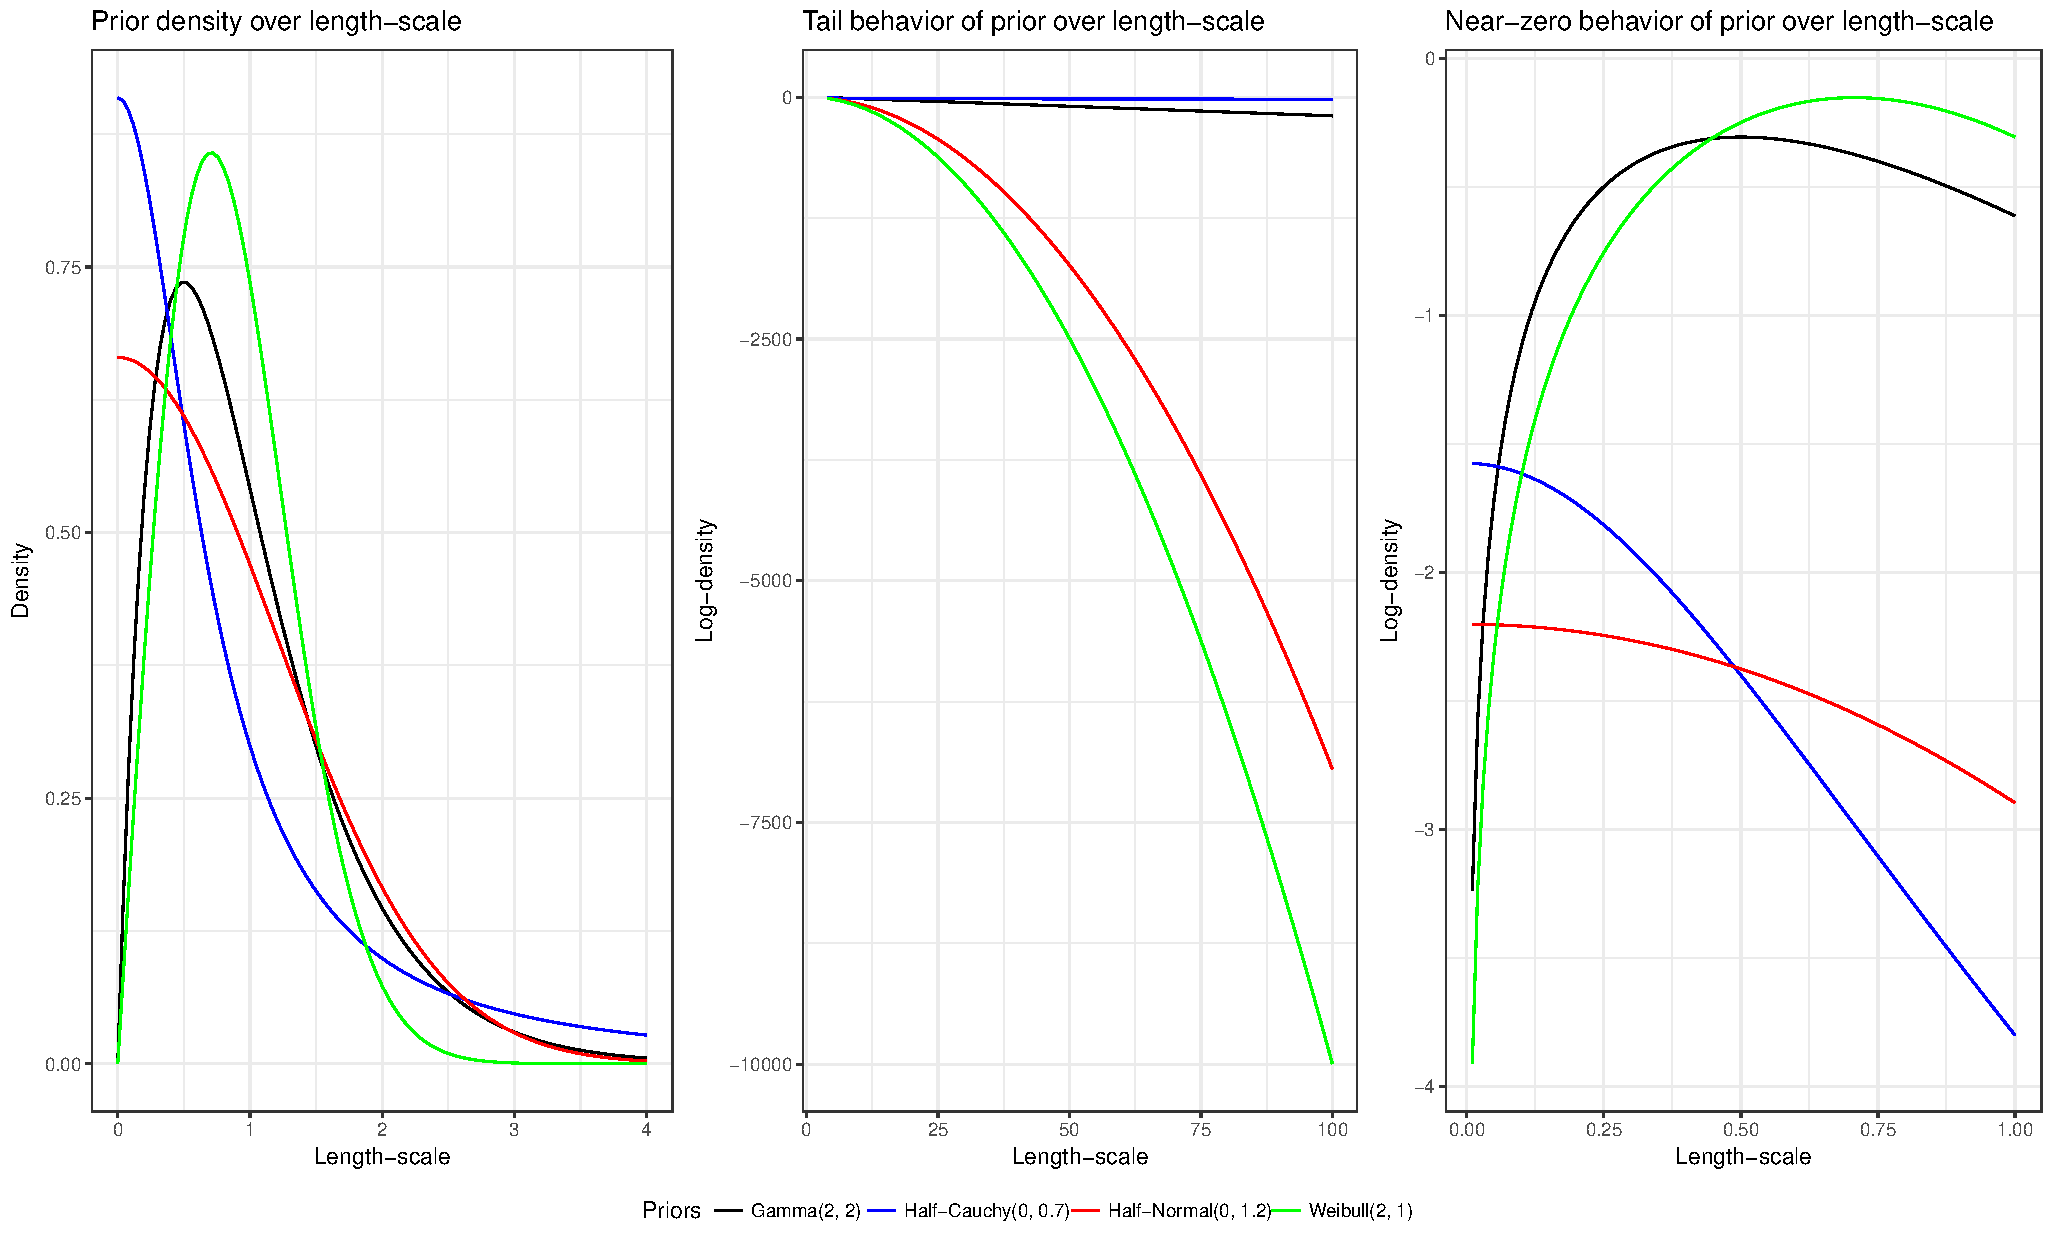
\includegraphics[width=100mm]{plots/prior_0_4_chart.pdf}
  \caption{Priors over $\ell$ (length-scale)}
\end{figure}

The $\text{Half-Cauchy}(0, 0.7)$ has the most mass at zero, and the most tail
mass. $\text{Gamma}(2, 2)$ has a heavy tail, but much lighter mass near zero
(in fact, it has zero mass exactly at zero, and thus is a zero-avoiding prior
\citet{gelman2014bayesian}). The $\text{Half-Normal}(0, 1.2)$ has a much lighter tail than
either the $\text{Half-Cauchy}(0, 0.7)$ or the $\text{Gamma}(2, 2)$, but still
has quite a bit of mass near zero. $\text{Weibull}(2, 1)$ has about as much
mass near zero as $\text{Gamma}(2, 2)$ but its tails are lighter than
$\text{Half-Normal}(0, 1.2)$.

We fix our priors for $\alpha$ and $\delta$ as $\text{Half-Normal}(0, 1)$.

\subsection{Datasets}

We simulated 100 datasets of 500 randomly sampled data points on the domain
from $[-2, 2]$ from a Gaussian process regression for 12 sets of parameters.
The data generating processes vary in the severity of the nonlinearity in the
Gaussian process prior, induced by scaling $\ell$ from near $0.04$ to $2.54$.
We then generated two sets of 100 replicated datasets at each $\ell$, one set
which had a signal-to-noise ratio $\alpha ^ 2/ \delta ^ 2$ (SN)
of $1$ and one set which had a
signal-to-noise ratio of $10$. The marginal variance $\alpha ^ 2 + \delta ^ 2$ was fixed at 1
for each parameter set. The full data set parameters are below:

\begin{table}[ht]
\centering
\begin{tabular}{rrrrrr}
  \hline
  & $\alpha$ & $\delta$ & SN & $\ell$ & $\Exp{C_0}$ \\ 
  \hline
1 & 0.71 & 0.71 & 1.00 & 2.54 & 0.50 \\ 
  2 & 0.95 & 0.30 & 10.00 & 2.54 & 0.50 \\ 
  3 & 0.71 & 0.71 & 1.00 & 1.27 & 1.00 \\ 
  4 & 0.95 & 0.30 & 10.00 & 1.27 & 1.00 \\ 
  5 & 0.71 & 0.71 & 1.00 & 0.64 & 2.00 \\ 
  6 & 0.95 & 0.30 & 10.00 & 0.64 & 2.00 \\ 
  7 & 0.71 & 0.71 & 1.00 & 0.40 & 3.16 \\ 
  8 & 0.95 & 0.30 & 10.00 & 0.40 & 3.16 \\ 
  9 & 0.71 & 0.71 & 1.00 & 0.13 & 10.00 \\ 
  10 & 0.95 & 0.30 & 10.00 & 0.13 & 10.00 \\ 
  11 & 0.71 & 0.71 & 1.00 & 0.04 & 31.62 \\ 
  12 & 0.95 & 0.30 & 10.00 & 0.04 & 31.62 \\ 
   \hline
\end{tabular}
\end{table}

\subsection{Inference}

We ran Stan on the command line (\citet{cmdstan}) for 1000 warmup and 1000
post-warmup iterations with 4 MCMC chains. All simulations run achieved Rhat <
1.05 for all parameters and achieved an acceptable effective sample size,as
suggested by \citet{gelman2014bayesian}.

\section{Results} \label{results}

We confirm the results of \citet{fuglstad2015interpretable} that in settings
with sparse data the tails of the posterior distribution under heavy-tailed
priors like the Cauchy are fat and can lead to biased inferences. An
illuminating example that arose from the setting in which the signal-to-noise
ratio was 1 and $\ell$ was set to 2.54 is worth highlighting.

The data and the latent mean functions are nearly constant across the $[-2,2]$
interval, as shown in $\ref{gp_set_3}$. Our inferences for $\ell$ and $\alpha$
are plotted in \ref{gp_set_3_len}. The Cauchy model has clear problems ruling
out the constant function in its posterior. This has implications for the 
posterior predictive mean distribution, which was biased sharply towards
constant functions, as can be seen in \ref{gp_set_3_post_pred_cauchy}. The
posterior predictive mean distribution from the $\text{Half-Normal}(0, 1.2)$
prior over $\ell$ is better, though we can see the model still having trouble
distinguishing the true latent mean function. This is to be expected in settings
where the signal-to-noise ratio is low and the data are not informative.

\begin{figure}[h] \label{gp_set_3}
  \centering
  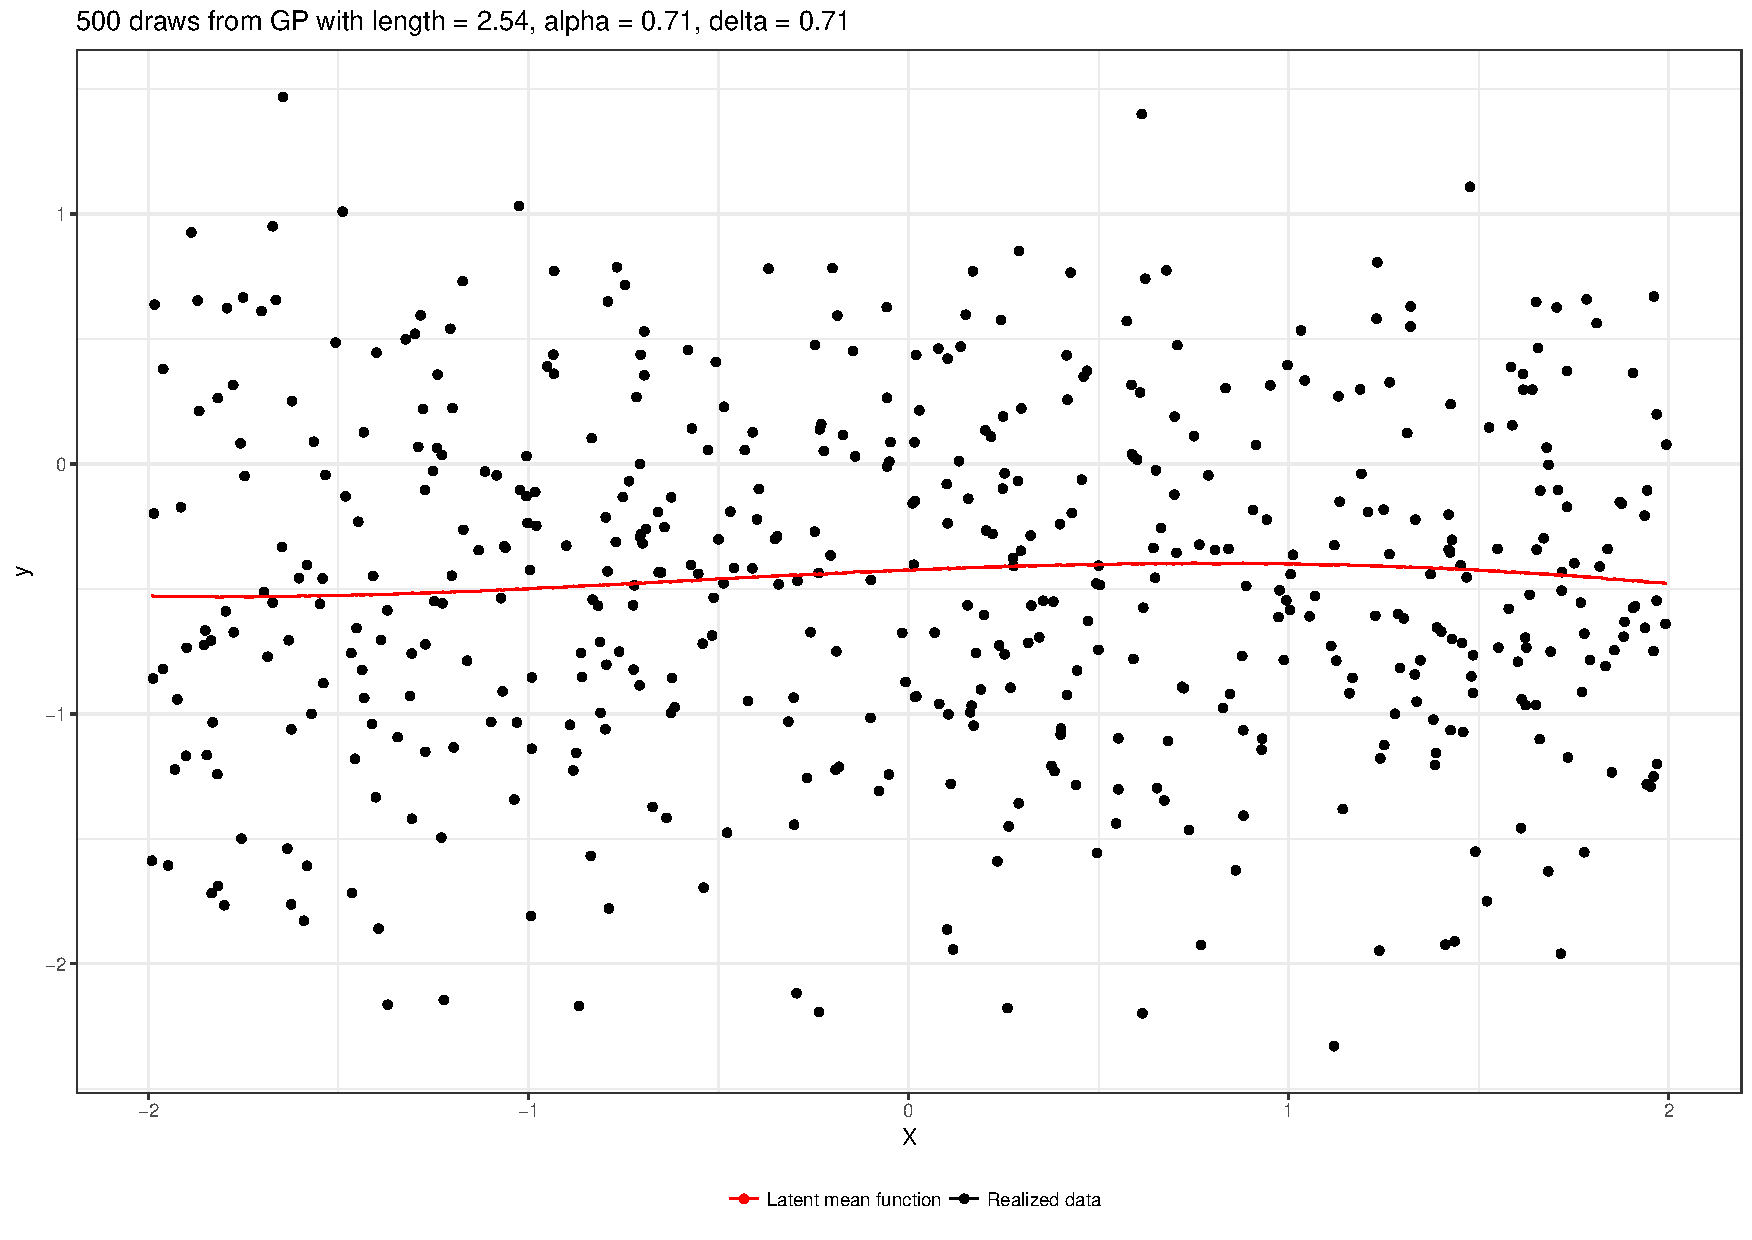
\includegraphics[width=100mm]{plots/dset_3_dgp.pdf}
  \caption{Synthetic dataset with nearly constant latent function and high noise}
\end{figure}

\begin{figure}[h] \label{gp_set_3_len}
  \centering
  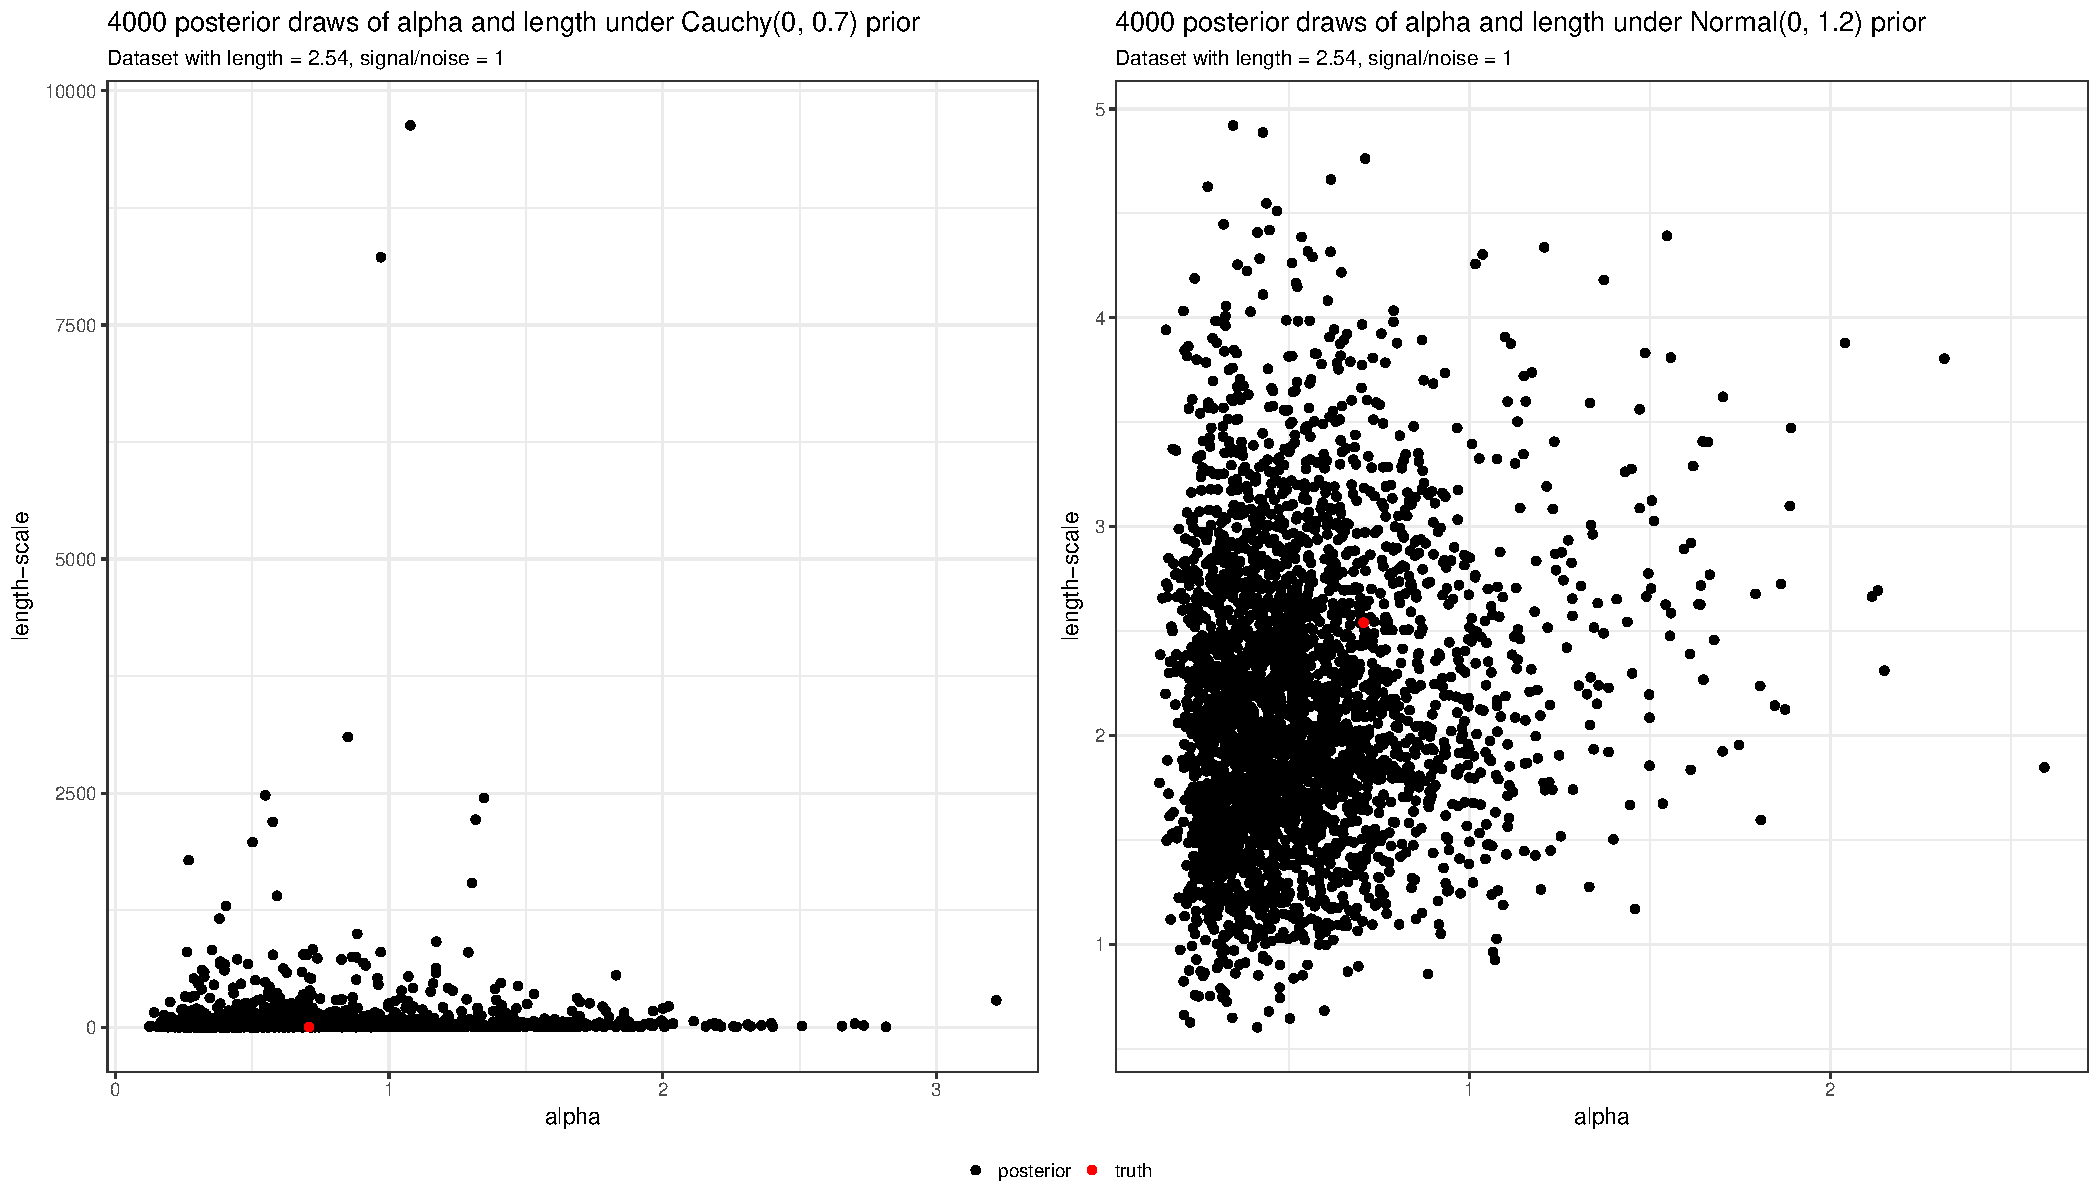
\includegraphics[width=100mm]{plots/dset_3_length_alpha.pdf}
  \caption{Posterior distributions for $\ell$ and $\alpha$ under
  $\text{Half-Cauchy}(0, 0.7)$ and $\text{Half-Normal}(0, 1.2)$ priors for $\ell$}
\end{figure}

\begin{figure}[h] \label{gp_set_3_post_pred_cauchy}
  \centering
  \includegraphics[width=100mm]{plots/half_cauchy_dset_3_post_pred_mean.pdf}
  \caption{4000 draws from the distribution of the posterior predictive means for new data over the $[-2,2]$ domain}
\end{figure}

Given that the $\text{Half-Cauchy}(0, 0.7)$ puts too much prior mass in the
tails of the distribution, and given that constant GPs and GPs that are
near-constant can be very hard to distinguish using any one data set, we
recommend against using the Cauchy when there are clear practical upper bounds
to $\ell$. The heavy tail of the Cauchy puts too much mass on data generating
processes that are indistinguishable from one another using finite data sets.

This can be seen in the distribution of posterior means for $\ell$ and $\alpha$
across simulations in the low signal-to-noise, large $\ell$ scenario in \ref{joint_len_alpha}. 

\begin{figure}[h] \label{joint_len_alpha}
  \centering
  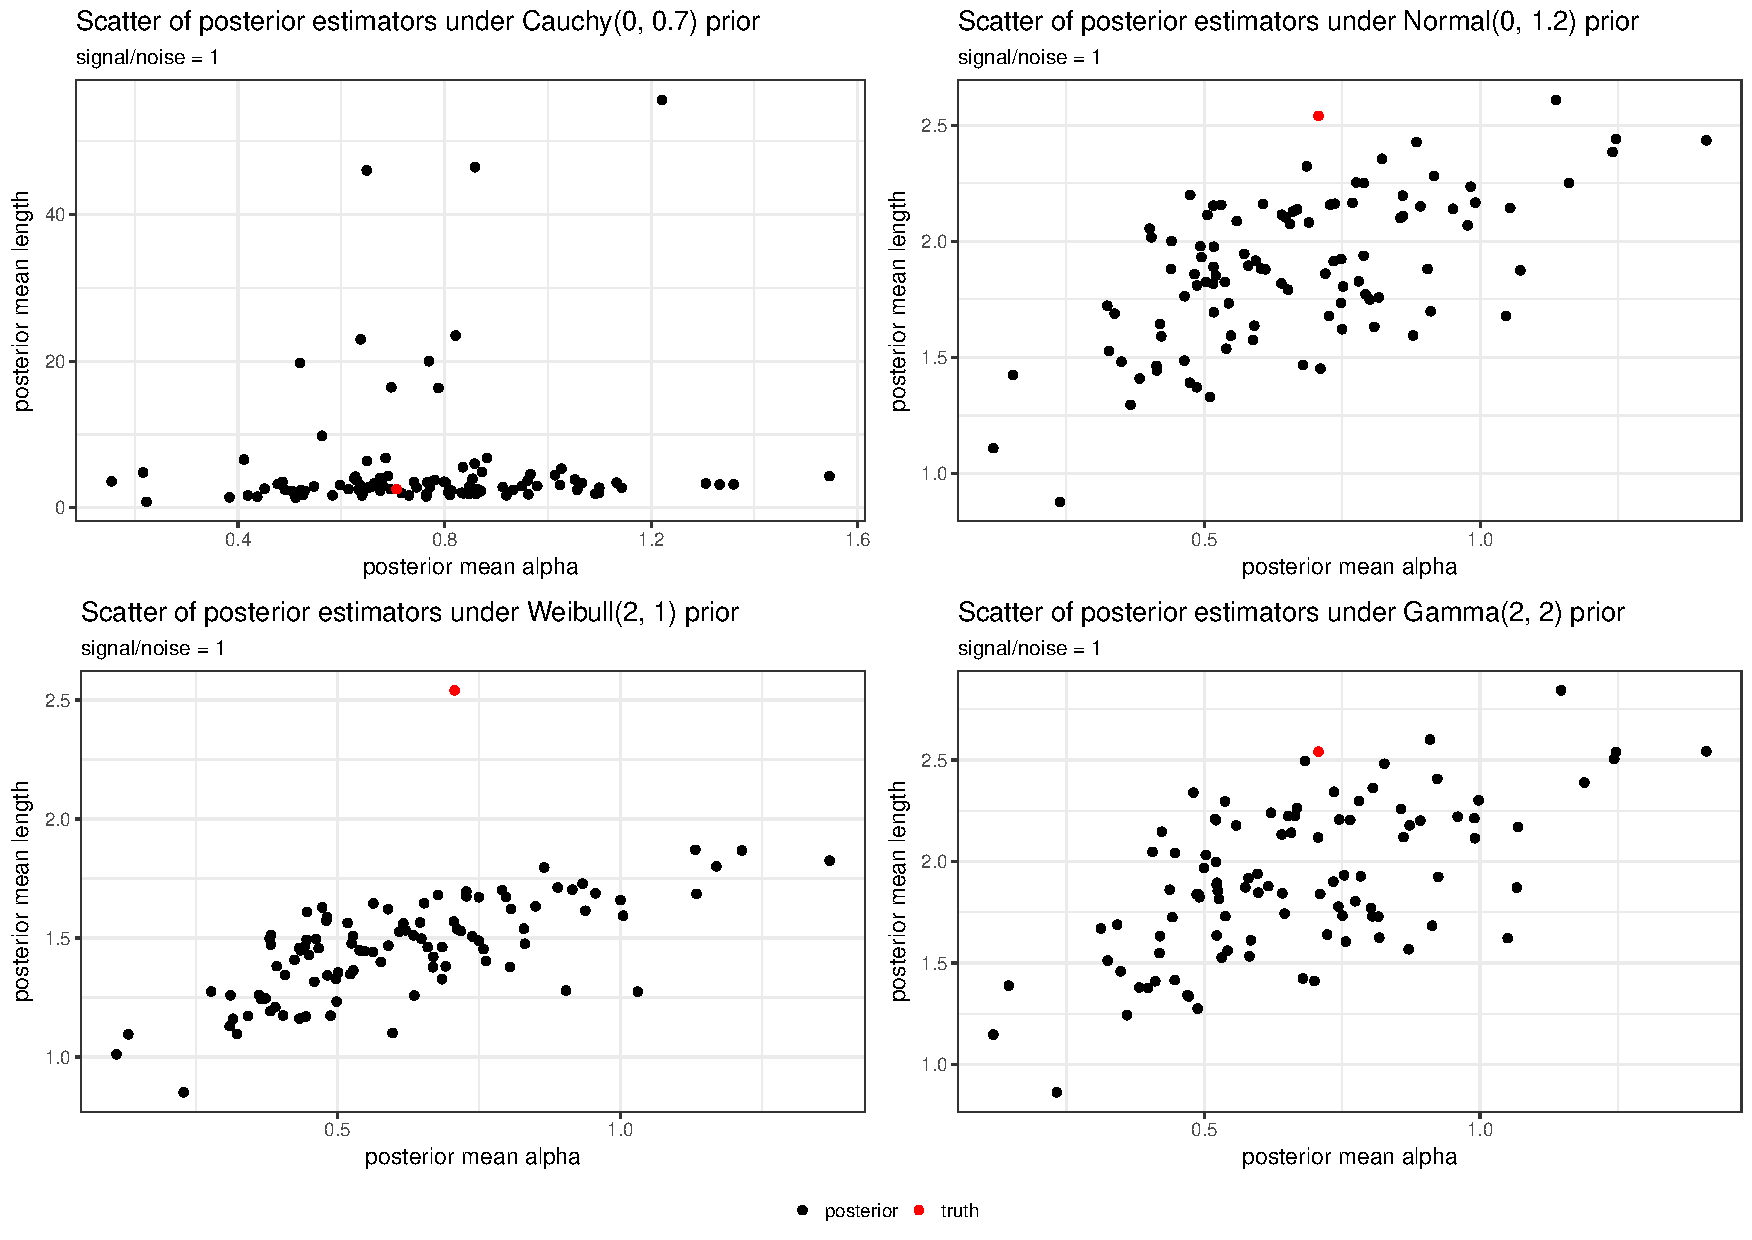
\includegraphics[width=100mm]{plots/dsets_2_5_alpha_0_7_alpha_length.pdf}
  \caption{Posterior means of $\alpha$ and $\ell$ under each prior}
\end{figure}

We can see the fat tails of the Half-Cauchy leading to biased estimates of
length-scale. Given the paucity of information in the data about the 
underlying mean function, the other priors have outsized effects on 
the posterior mean estimates for $\ell$. The correlation in the posterior
means between simulations also mirrors posterior correlation within 
simulations between draws of length-scale $\ell$ and draws of $\alpha$.

Under the data generating processes that had shorter length-scales and low 
signal-to-noise, we do not see the contrary problem with priors that have mass
at zero leading to posteriors that place mass on zero. This is likely a
function of the data being dense. We do see strong positive correlation between
$\ell$ and $\alpha$. 

\begin{figure}[h] \label{joint_len_alpha_high_SN}
  \centering
  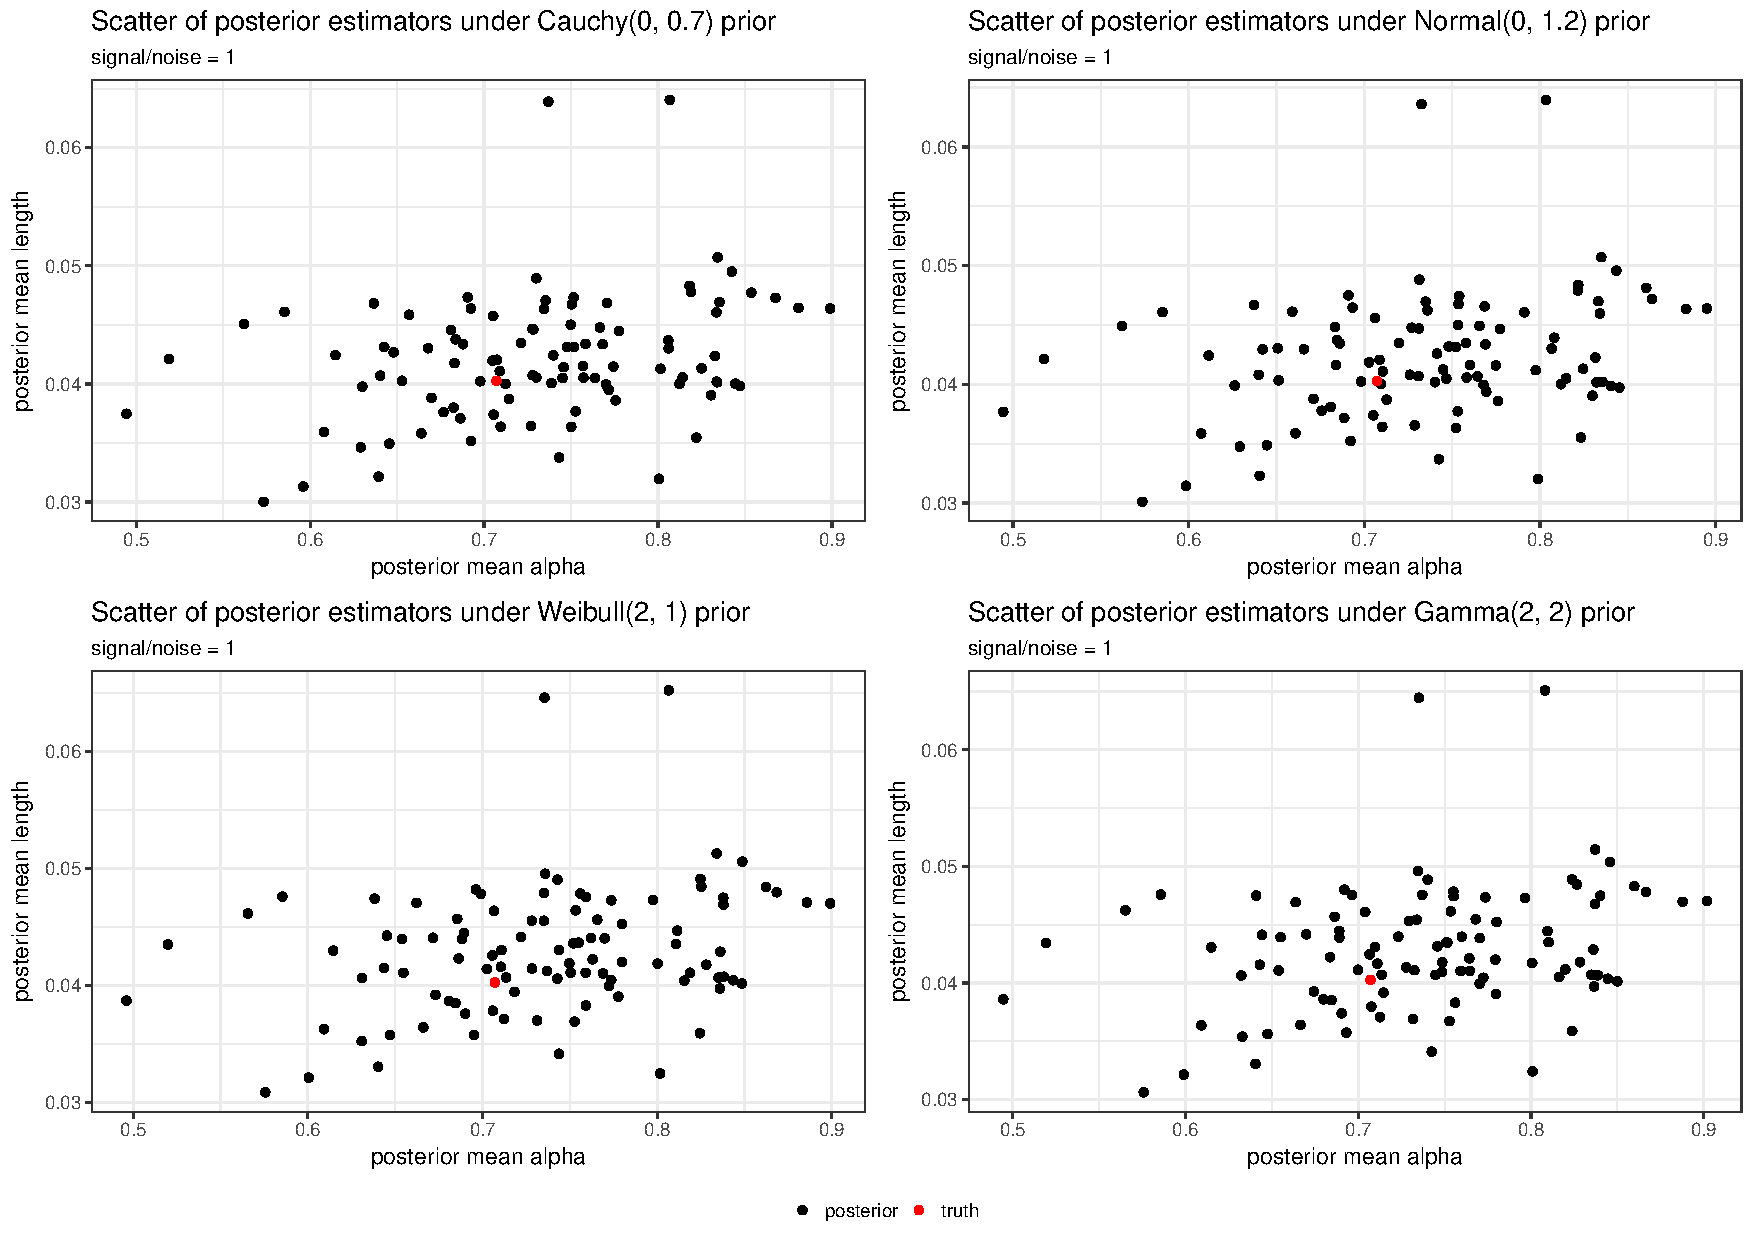
\includegraphics[width=100mm]{plots/dsets_0_05_alpha_0_7_alpha_length.pdf}
  \caption{Posterior means of $\alpha$ and $\ell$ under each prior}
\end{figure}

These experiments suggest that setting a soft upper bound on $\ell$ with a 
prior with a fast-decaying tail is a good weakly informative prior. More work needs 
to be done to understand joint priors over $\alpha$, $\delta$, and $\ell$.

\pagebreak

\section{Appendix}

\subsection{Stan code}

\begin{verbatim}
data {
  int<lower=1> D;
  int<lower=1> N;
  int<lower=1> N_pred;
  real x[N];
  vector[N] y;
  real x_pred[N_pred];
}
transformed data {
  vector[N] mu;
  matrix[N_pred, N_pred] nug_pred;

  mu = rep_vector(0, N);
  nug_pred = diag_matrix(rep_vector(1e-5,N_pred));
}
parameters {
  real<lower=0> length;
  real<lower=0> alpha;
  real<lower=0> delta;
}
model {
  matrix[N, N] L_Sigma;
  {
    matrix[N, N] Sigma;
    Sigma = cov_exp_quad(x, alpha, length);
    for (n in 1:N)
      Sigma[n, n] = Sigma[n,n] + delta;
    L_Sigma = cholesky_decompose(Sigma);
  }
  length ~ gamma(2, 2);
  delta ~ normal(0, 1);
  alpha ~ normal(0, 1);

  y ~ multi_normal_cholesky(mu, L_Sigma);
}
generated quantities {
  vector[N_pred] f_pred;

  {
    matrix[N, N] L_Sigma;
    vector[N] K_div_y;
    matrix[N, N_pred] k_x_x_pred;
    matrix[N, N_pred] v_pred;
    matrix[N_pred, N_pred] cov_f_pred;
    {
      matrix[N, N] Sigma;
      Sigma = cov_exp_quad(x, alpha, length);
      for (n in 1:N)
        Sigma[n, n] = Sigma[n,n] + delta;
      L_Sigma = cholesky_decompose(Sigma);
    }
    K_div_y = mdivide_left_tri_low(L_Sigma, y);
    K_div_y = mdivide_right_tri_low(K_div_y',L_Sigma)';
    k_x_x_pred = cov_exp_quad(x, x_pred, alpha, length);
    f_pred = k_x_x_pred' * K_div_y; 
    v_pred = mdivide_left_tri_low(L_Sigma, k_x_x_pred);
    cov_f_pred = cov_exp_quad(x_pred, alpha, length) - v_pred' * v_pred;

    f_pred = multi_normal_rng(f_pred, cov_f_pred + nug_pred);
  }
}
\end{verbatim}


\bibliographystyle{plainnat}
\bibliography{bib_inf_priors}

\end{document}
